\section{Test af reverb og echo impulsrespons}\label{sec:test_af_effekt}
Da echo og reverb begge er tidsinvariante effekter betyder det, at de kan karakteriseres af deres impulsrespons.
For at sammenligne med teorien opsattes der simulink modeller med anti-aliasing- og rekonstruktionsfiltrenes overføringsfunktion på hhv. signalinput og output.
\begin{figure}[!ht]
	\centering
	\begin{minipage}{0.50\textwidth}
		\centering
		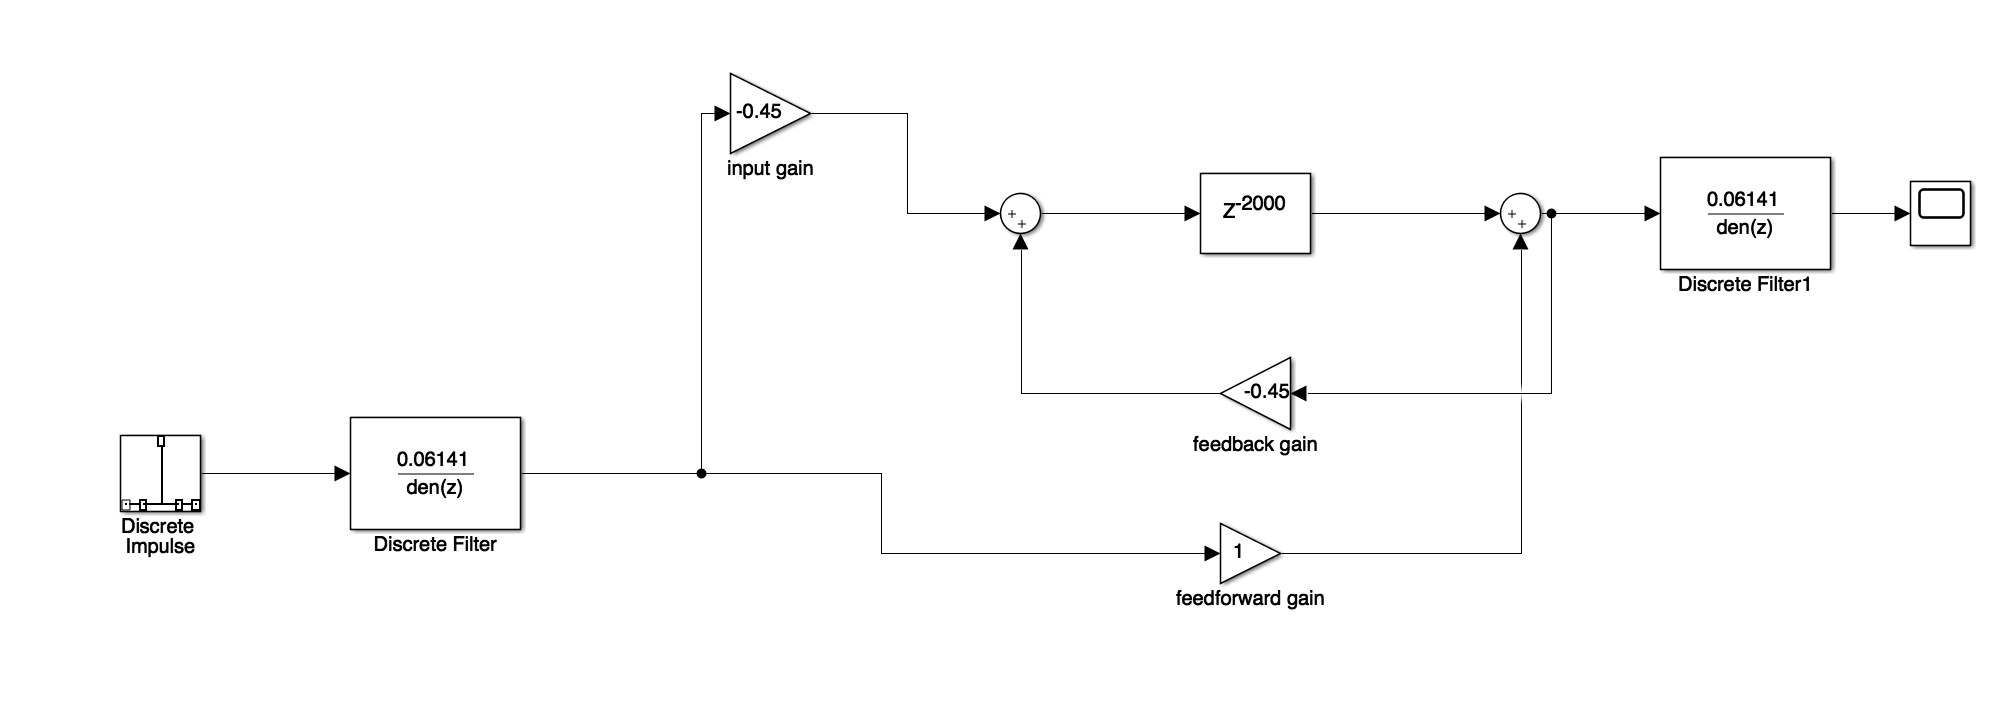
\includegraphics[width=0.9\textwidth, height=5cm]{billeder/reverb-testopsaetning.png}
		\caption{Simulink reverb model}
		\end{minipage}\hfill
	\begin{minipage}{0.50\textwidth}
		\centering
		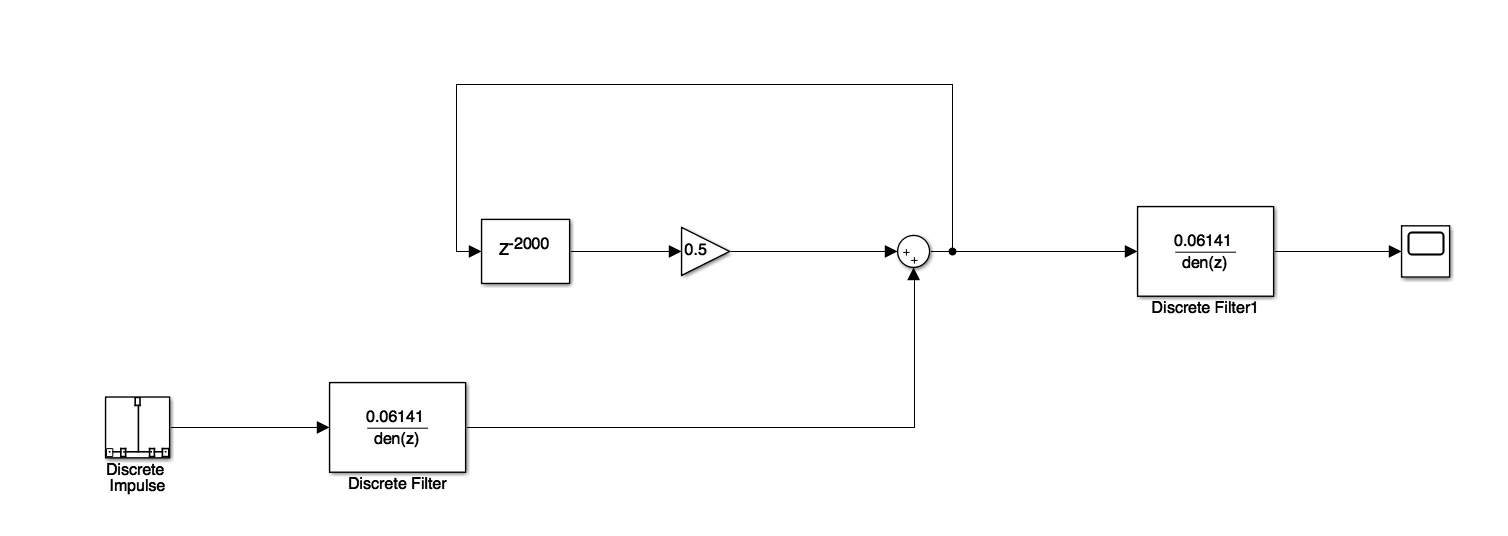
\includegraphics[width=0.9\textwidth, height=5 cm]{billeder/echo-testopsaetning.png}
		\caption{Simulink echo model}
		\end{minipage}
\end{figure}

\section{Fremgangsmetode}
Der blev koblet en funktionsgenerator på signalindgangen, og funktionen ''pulse`` valgtes som funktion med en amplitude på $750\si{mV}$ og et DC-offset på $500\si{mV}$ for at matche biaset på opampsne på udgangen. %noget om biaset evt.
På signaloutputtet blev der tilsluttet en load på $XXX\si{k\Omega}$. \husk{Indsæt rigtig værdi på load modstanden}
Oscilloskopet sattes til ''single sweep`` med en trigger på $750\si{mV}$.
Reverbeffekten blev sat til at have et delay på $z^{-2000}$ og input- og feedbackgainet blev begge sat til $-0.45$.\newline
På echoeffekten blev delayet sat til $z^{-2000}$ og feedbackgainet blev sat til $0.5$.
\subsection{Resultat}
